\documentclass{article}
\usepackage[utf8]{inputenc}
\usepackage{placeins}
\usepackage{caption}        % better captions
\usepackage{subcaption}     % for subfigures
\title{MPI:Course}
\author{Oliver Siig, Sudarshan Vijay}
\date{26th of January 2020}

\usepackage{natbib}
\usepackage{graphicx}

\begin{document}

\maketitle

\section{Bandwidth and latency estimation}

In order to measure the bandwidth and latency of the processors available on gbar, a simple piece of code was implemented, which sent an array containing double precision numbers from one processor to another and back again. This was tested for a number of array sizes from $2^{0}$ to $2^{16}$, with each array being tested 10 times. The results from this is summarized in table \ref{tab:bandwidth} below. While this is not clear from the table, the raw data shows that the processor of rank 1 is generally slightly slower than rank 0. This processor is the one which first receives and then sends data.\\

\begin{table}[!h]
\caption{Transmission times for data array transfer}
\label{tab:bandwidth}
\centering
\begin{tabular}{|l|l|l|l|}
\hline
Size & Minimum  & Maximum  & Average  \\ \hline
$2^{0}$  & 2.27E-05 & 2.89E-05 & 2.56E-05 \\ \hline
$2^{2}$  & 2.24E-05 & 2.98E-05 & 2.57E-05 \\ \hline
$2^{4}$  & 2.26E-05 & 2.86E-05 & 2.53E-05 \\ \hline
$2^{6}$  & 5.67E-05 & 7.02E-05 & 6.04E-05 \\ \hline
$2^{8}$  & 6.30E-05 & 7.38E-05 & 6.63E-05 \\ \hline
$2^{10}$ & 1.19E-04 & 1.35E-04 & 1.24E-04 \\ \hline
$2^{12}$ & 1.31E-04 & 1.46E-04 & 1.36E-04 \\ \hline
$2^{14}$ & 2.22E-04 & 2.35E-04 & 2.27E-04 \\ \hline
$2^{16}$ & 5.20E-04 & 5.35E-04 & 5.29E-04 \\ \hline
$2^{18}$ & 1.68E-03 & 1.70E-03 & 1.68E-03 \\ \hline
\end{tabular}
\end{table}
 The average time as a function of array size is also illustrated graphically in figure \ref{fig:bandwidth}. The total time is assumed to be divided into two parts:
 \begin{equation}
     T(n) = T_{latency} + n/bandwidth
 \end{equation}
 where $n$ is the data size. In theory both bandwidth and latency could be determined from a linear fit of all data points, with the bandwidth given as 1/slope and latency as the y-intercept. It is clear from the figure however, that there is no clear linear relationship. Particularly from the logarithmic plot in figure \ref{fig:logplot}, it is seen that there is no slowdown going from $2^0$ to $2^4$. Instead, these array sizes seem to be completely dominated by latency, and the latency is estimated to be 2.56E-05 s, taking the average of the 3 systems. For the larger arrays it does however appear that there is a linear relationship. A linear fit of the values from $2^{12}$ to $2^{18}$ is shown in figure \ref{fig:linear} with a slope of 7.45E-10, corresponding to a bandwidth of 1.34GB/s.
\begin{figure}[h]
\centering
\begin{subfigure}{.49\textwidth}
  \centering
  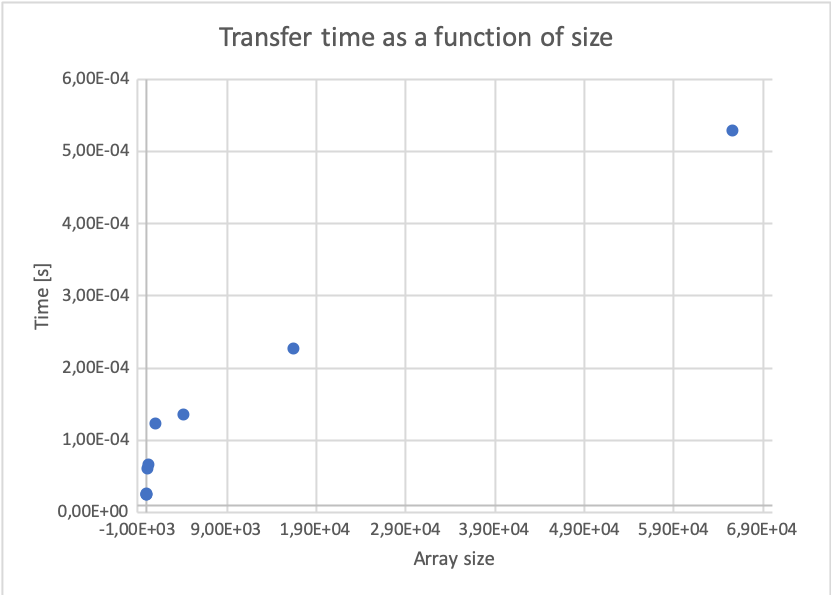
\includegraphics[width=1\linewidth]{figures/normplot.png}
  \caption{Proportional axes}
  \label{fig:normplot}
\end{subfigure}%
\begin{subfigure}{.49\textwidth}
  \centering
  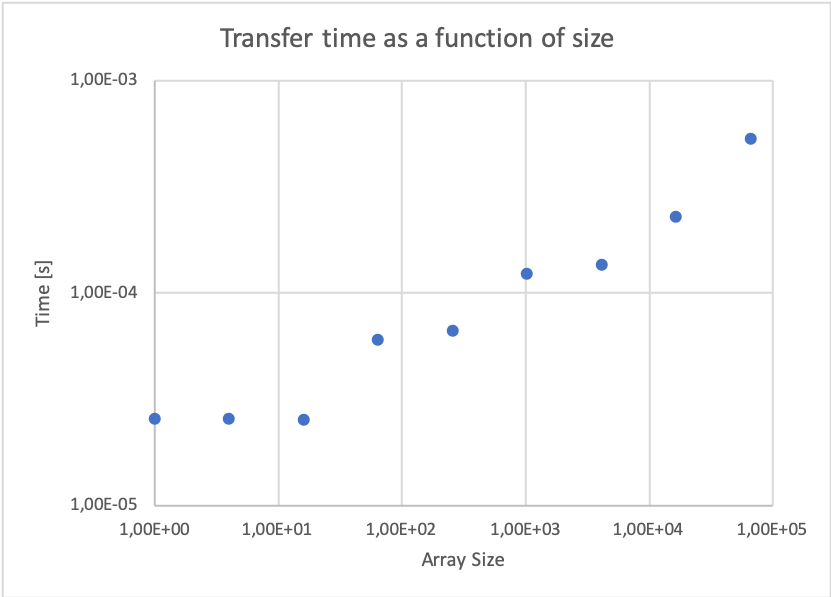
\includegraphics[width=1\linewidth]{figures/logplot.png}
  \caption{Logarithmic axes}
  \label{fig:logplot}
\end{subfigure}
\caption{Plot of the transmission time as a function of array length from $2^0$ to $2^{18}$ double-precision numbers.}
\label{fig:bandwidth}
\end{figure}

\begin{figure}[!h]
    \centering
    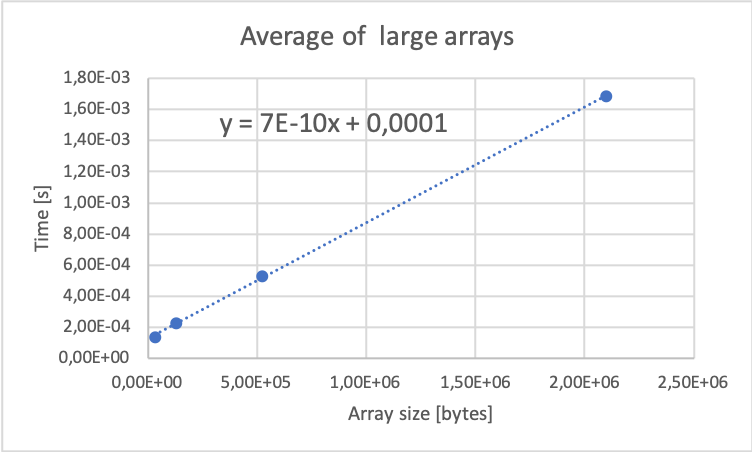
\includegraphics[width=8cm]{figures/linearplot.png}
    \caption{Plot of the data points that exhibit a linear correlation. The time, given in seconds, is shown as a function of data amount, given in bytes. The slope correponds to the inverse bandwidth.}
    \label{fig:linear}
\end{figure}

\section{MPI Diffusion problem}

The code consists of the main program $T_diffusion.f90$. There are four submodules that are called

\begin{verbatim}
CALL vars(Lx, Ly, Nx, Ny, D_coeff, dt, n_steps, spec, steps)

CALL init(Lx, Ly, Nx, Ny, D_coeff,dx,dy,dt,T_trix,T_trix_new,
Nxloc,Nyloc,Nbound,rdx,rdy)

CALL data(Nxloc,Nyloc,Nbound,D_coeff,n_steps,rdx,rdy,dt,
T_trix,T_trix_new)

CALL write(Nxloc, Nyloc, Nbound, dx, dy, T_trix, steps, Nx, Ny)
\end{verbatim}

The init module splits the matrix based on the rank of the process. The last process always takes whatever grid points are left. MPI is initialized within this submodule

\begin{verbatim}
    IF (irank==isize-1) THEN
        ALLOCATE(T_trix(Nxrem+1,Nyloc))
        ALLOCATE(T_trix_new(Nxrem+1,Nyloc))
        Nbound=Nxrem
\end{verbatim}

Communication is carried out by the data module. This passes information forward, with each sub-matrix sending from the last dummy row and receiving to the first dummy row. The first chunk only sends, while the last only receives. 

\begin{verbatim}
      IF ( isize > 1) THEN
    ! MPI related commands
    IF ( irank .EQ. 0 ) THEN
     ! This is the first process only send
     dest = irank + 1
     CALL MPI_Send(T_trix_new(Nbound,:), Ny, MPI_DOUBLE_PRECISION, dest, tag1, &
             MPI_COMM_WORLD, ierror)
    ELSEIF ( irank .EQ. isize-1 ) THEN
      ! This is the last process only receive
      srank = irank - 1
      CALL MPI_Recv( T_trix_new(1,:), Ny, MPI_DOUBLE_PRECISION, srank, tag2, &
            MPI_COMM_WORLD, status_mpi, ierror)
    ELSE
      ! Processor in the middle sends and receives
      dest = irank + 1
      srank = irank - 1
      CALL MPI_SendRecv( T_trix_new(Nbound,:), Ny, MPI_DOUBLE_PRECISION, dest, tag1, &
      T_trix_new(1,:), Ny, MPI_DOUBLE_PRECISION, srank, tag2, MPI_COMM_WORLD, &
      status_mpi, ierror)
    ENDIF
\end{verbatim}

The reverse happens in the case of the second communication.


The Root mean square value was computed for a 4097x4097 matrix using 4 cores. This was compared to that case of a serial run. It was found that the root mean square error was 0.000328450832754


Parallel efficiency and speedup was computed for the same matrix used above. The number of cores used was 1, 2, 4, 8. 

The speedup was calculated by 

\begin{equation}
    S(Nproc) = \frac{t(1)}{max(t_{i})} \frac{N(Nproc)}{N}
\end{equation}

and the parallel efficiency was calculated by 

\begin{equation}
    E(Nproc) = S(Nproc) / Nproc
\end{equation}

\begin{figure}
    \centering
    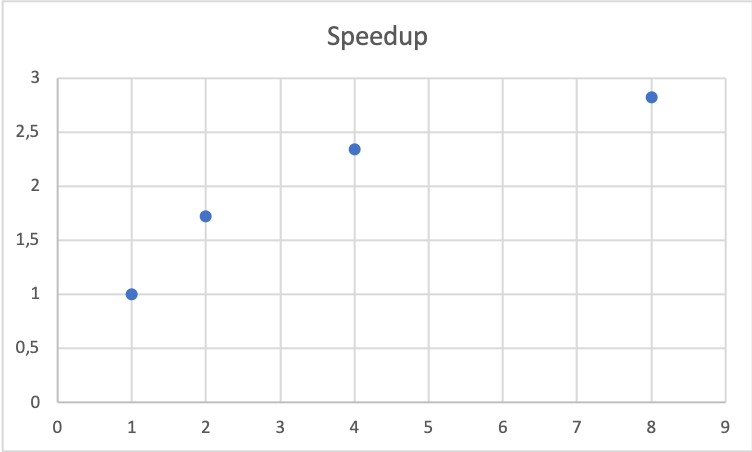
\includegraphics[width=8cm]{figures/speedup_diff.png}
    \caption{Speedup for Diffusion program}
    \label{fig:my_label}
\end{figure}

\begin{figure}
    \centering
    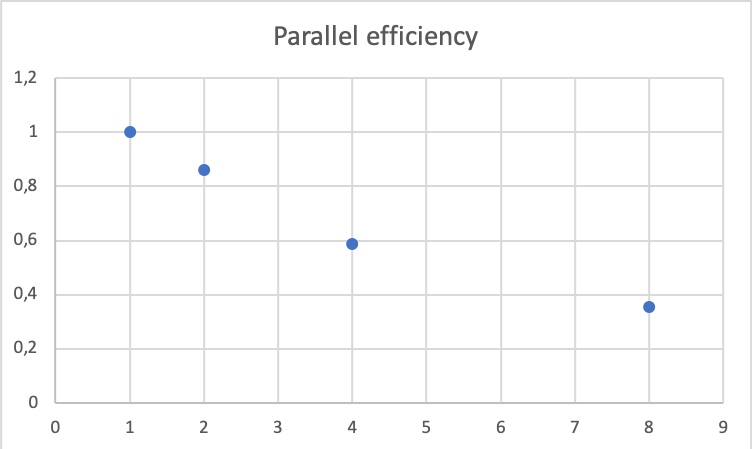
\includegraphics[width=8cm]{figures/parallel_efficiency_diff.png}
    \caption{Parallel efficiency for Diffusion program}
    \label{fig:my_label}
\end{figure}




\end{document}
